% -> 怎么创建对象
%     -> new Object()
%     -> 字面量
%     -> 工厂函数
% -> 构造函数
% -> 练习

\chapter{使用\,JavaScript\,对象}

本章要点:

\begin{itemize}
\item 根据需要抽取对象的属性与方法
\item 利用对象的动态特征创建对象
\item 利用对象字面量创建对象
\item 利用工厂函数(工厂设计模式)来创建对象
\item 利用构造函数来创建对象
\end{itemize}


\section{怎么创建对象}

前面我们已经了解到, 面向对象编程就是使用对象进行开发. 而且我们已经使用``名词提炼法''提取出了对象.
现在我们需要深入的是对象里面应该有哪些成员属性以及成员方法. 首先我们来解释``属性'', ``方法''这两个名词.

我们知道对象是将数据与操作数据的功能打包到一起. 数据可以是基本类型(数字\,\lstinline|number|, 
字符串\,\lstinline|string|, 或布尔值\,\lstinline|boolean|), 也可以是其他对象或者函数. 
我们将保存的数据称为对象的属性(\,property\,), 将保存的函数称为对象的方法(\,method\,).

在\,JavaScript\,中, 函数是一等公民, 函数也是一种数据类型. 与其他类型一样, 可以被赋值, 被函数传递与返回.
这里我们暂时不讨论这个问题, 后面我们会详细说明.

因此抽象一下, 将函数与基本类型, 对象都看成数据的话, JavaScript\,中, 对象就是键值对的集合%
%
\footnote{对象这个词很抽象, 这里专门指\,JavaScript\,中的对象类型. 后文中如果不加特殊说明, 均指对象类型}. 
%
即包含一个或多个键值对的结构. 实际上, 作为对象有多种表现形式. 

例如: \lstinline|Math|\,对象, 它提供了大量的数学方法, 
使用的时候不需要做任何处理, 直接调用其方法. 这样的对象就是功能集(方法集), 
其目录就是为了整合方法, 便于维护, 管理与调用.

再比如, 我们使用的较多的\,\lstinline|DOM|\,对象, 它是集方法与数据与一身. 数据用于描述其属性, 显示的文本或样式等,
而方法用于操作\,\lstinline|DOM|\,节点之间的关系(追加节点, 移除节点, 查询等操作).

又如为了保存多个数据使用的数组, 或键值对\footnote{例如: \lstinline|\{name:'jiangkun',age:19,gender:'male'\}|.}.
它便是为了保存数据, 管理数据而存在. 一般不会为其添加方法, 它仅仅是为了存储数据.

因此创建对象首先要确定对象有哪些属性, 然后定义该属性, 给它提供数据. 
然后再讨论这个对象有什么功能, 就定义什么方法(方法就是函数的特例), 为其提供函数代码.
那么我们研究的对象的那么多属性与功能, 我们又该如何抽取呢? 需要哪些属性? 需要提供什么方法? 
所以我们首先来看看对象的``抽象性''的概念.

\subsection{抽象性描述}

抽象性(\,abstraction\,), 就是指关注我们需要关注的特征与能力. 例如, 我们要做一个电商的站点.
我们的每一个商品都是我们的对象. 以买书为例. 书本即为我们研究的对象, 但是我们需要关注的是书本的那些特征呢?
书本有名字, 出版社, 作者等信息, 除此之外还有尺寸, 纸张类型, 重量, 价格, ISBN\,编号等.
如果我们只是完成一个产品描述, 上述信息已经足够, 但是书本的特征不仅仅是这一些. 如图\,\ref{ch02_0001}, 
书本所描述的信息还有主要内容说明, 作者简介, 来自于各方的简评, 以及出版社联系方式等等. 
还有很多相关的数据.

\begin{figure}[!htbp]
\centering
\noindent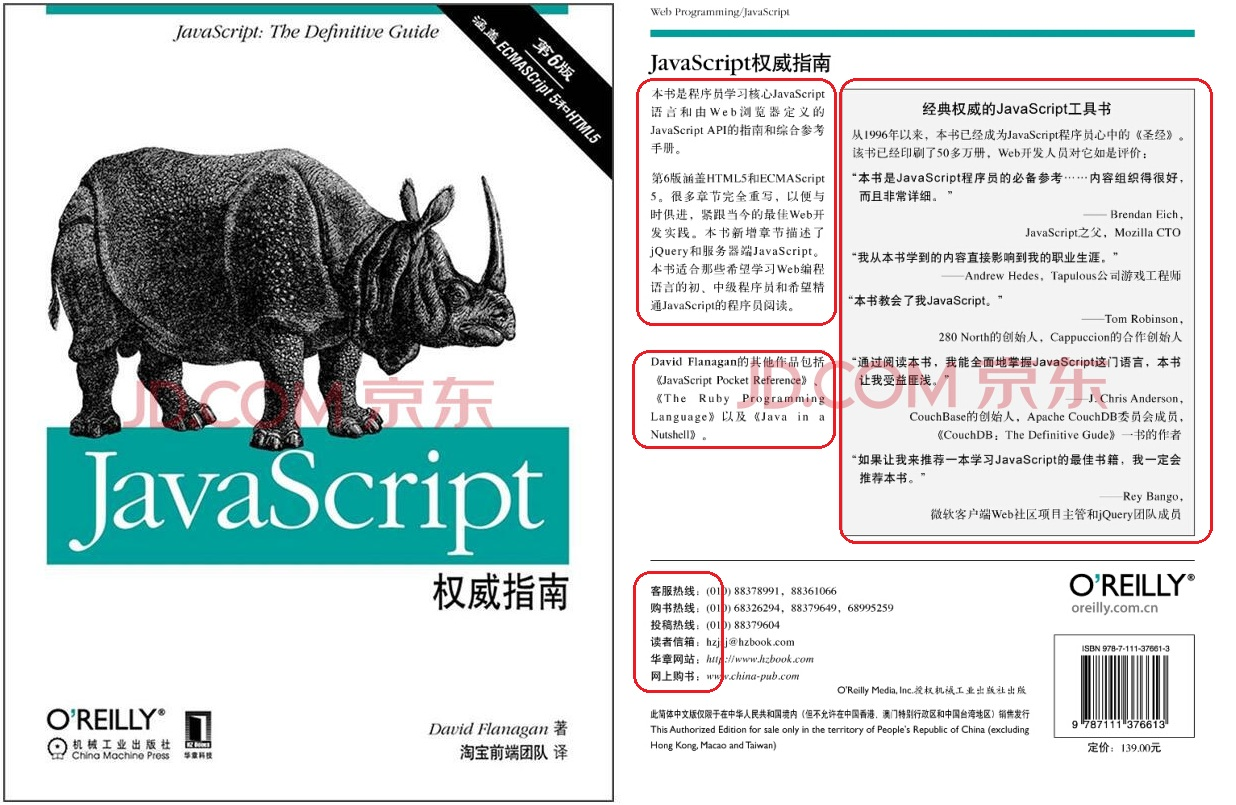
\includegraphics[width=\textwidth]{imgs/jsqwznv6.jpg}
\caption{书本封面示例\label{ch02_0001}}
\end{figure}

但是描述书本的信息不用那么多. 简单点, 做\,demo\,的时候甚至只需要书名, 作者, 价格, 出版社, 以及一张封面图片即可.

那么又有问题了: 一张音乐\,CD\,需要描述的信息基本上也是: 专辑名称, 演唱者, 价格, 发行商, 已经专辑封面. 互相比较一下. 
仅仅通过数据是没有办法准确描述这个具体事物的. 但是作为我们研究的电商项目, 作为商品已经足够了. 这便是抽象性(\,abstraction\,).

抽象讲究的感觉是不准确, 有概括性. 而在上面的描述中, 仅仅通过数据, 没有办法准确的将事物描述清晰. 
这一特点恰好便是抽象性. 一句话: \emph{在没有确定描述的大条件下, 仅仅通过数据, 没有办法准确描述具体的事物}. 
好比``张三'', ``男'', 10. 这几个数据可以描述什么呢? 一个人, 一个受人喜爱的公仔, 甚至是一只小狗或小猫等. 
这就是抽象性. 

那么如何在代码中体现出来呢? 很简单, 抽取属性与方法的时候, 只关注我们想要关心的属性与功能. 
\footnote{任何一种属性的抽取方式都没有正确与错误, 只有更加合适一说. 要抽取什么属性或方法, 这一点有时需要一个度, 需要在不断积累中慢慢掌握.}

\subsection{使用\,\lstinline|new Object()|\,来创建对象}

\subsection{使用对象的字面量(\,literal\,)来创建对象}

\subsection{使用工厂函数(\,factory function\,)来创建对象}



\section{构造函数}

\subsection{构造函数的语法}

\subsection{使用构造函数创建对象}

\subsection{相关概念}

\section{案例}
